\documentclass{article}

\textwidth=6.5in
\textheight=8.5in
\voffset=-54pt
\oddsidemargin=0in
\evensidemargin=0in
\setlength{\parskip}{8pt}
\setlength{\parindent}{0pt}

\usepackage{amsmath, amssymb}
\usepackage{ifthen}

\usepackage[inline]{enumitem}
\setlist{topsep=0pt, parsep=8pt}

\usepackage[rgb,table]{xcolor}\convertcolorsUfalse
\usepackage{graphicx}

% change hyperref options
\PassOptionsToPackage{hyphens}{url}
\usepackage[bookmarks,colorlinks,linkcolor=black,citecolor=blue,pdfstartview=FitH,urlcolor=blue]{hyperref}
\hypersetup{pdfpagemode=UseNone}
\usepackage{bookmark}

\usepackage{graphicx}
\usepackage{multicol}
\usepackage{framed}
\usepackage{array}

\usepackage{icomma}

\usepackage{marginnote}
\usepackage[colorinlistoftodos]{todonotes}
\renewcommand{\marginpar}{\marginnote}

\usepackage{soul}

\usepackage{pgfplots}
\pgfplotsset{compat=1.18}  
\pgfplotscreateplotcyclelist{mycolor}{black, blue, red, green!70!black, magenta, purple, cyan, orange }  
\pgfplotsset{
  disabledatascaling,
  cycle list=tikzcolor, 
  axis lines=middle,
  every axis plot/.style={no marks, thick},
  every axis/.style={
    enlarge x limits=false,
    enlarge y limits=auto,
    xlabel style={at={(current axis.right of origin)},anchor=west},
    ylabel style={at={(current axis.above origin)},anchor=south},
    % extra x and y ticks for asymptotes
    extra x tick style={grid=major, grid style={dashed,black}},
    extra y tick style={grid=major, grid style={dashed,black}},
    /pgf/number format/1000 sep={},
  },    
  tick label style = {font=\footnotesize, fill=\currentbgcolor, inner sep=0pt},    
  xticklabel shift=1pt,    
  scaled ticks=false,
  scaled y ticks=false,
  unbounded coords=jump,
  samples=101,
  minor tick length=0,
  scatter/classes={
    open={mark=*,draw=black,fill=white, mark size=2, thin},
    closed={mark=*,draw=black,fill=black, mark size=2, thin}
  },
  width=3in,
}
\pgfplotsset{open/.style={only marks, mark=*, fill=white, thin, mark size=2}}
\pgfplotsset{closed/.style={only marks, mark=*, draw=black, fill=black,
    thin, mark size=2}}
\pgfplotsset{labeled/.style={nodes near coords, only marks, mark=*, draw=black, fill=black, thin, mark size=2, point meta=explicit symbolic}}

\pgfplotsset{gridgraph/.style={clip=false, axis line style={shorten
      >=-8pt}, xlabel style={xshift=8pt}, ylabel style={yshift=8pt},
    enlargelimits=false, grid=major, tick style={black}}} 

\usepackage{tikz}
\usetikzlibrary{
  matrix,%
  % enables the snake paths
  decorations.pathmorphing,%
  % enables bigger arrows
  decorations.markings,%
  decorations.pathreplacing,%
  decorations.text,%
  calc,%
  patterns,%
  shapes.geometric,%
  arrows,
  decorations.shapes,
  positioning,
  plotmarks,
  intersections
}
\tikzset{>=latex} % sets default arrow type in tikz
\tikzset{font=\normalsize}
\tikzset{mark size=1.5pt, mark options=thin}
\tikzset{pin distance=4pt,
  every pin edge/.style={<-, thin, shorten <= -2pt}}

\interfootnotelinepenalty=10000
\renewcommand{\thefootnote}{(\arabic{footnote})}

\usepackage{multirow, bigdelim}

% change to \usepackage[sols]{handout} to see solutions
\usepackage[]{handout}

\newcommand\iscurrentenumi[1]{%
  \ifthenelse{\equal{#1}{\theenumi}}{}{#1}}
\setenumerate[1]{ref=\#\arabic*}
\setenumerate[2]{ref=\protect\iscurrentenumi{\theenumi}(\alph*)}
\newcommand\enumiiprefix[2]{%
  \ifthenelse{{\equal{#1}{\theenumi}}\AND{\equal{#2}{(\alph{enumii})}}}{}{}%
  \ifthenelse{{\equal{#1}{\theenumi}}\AND{\NOT{\equal{#2}{(\alph{enumii})}}}}{#2}{}%
  \ifthenelse{\equal{#1}{\theenumi}}{}{#1#2}%
}
\setenumerate[3]{ref=\protect\enumiiprefix{\theenumi}{(\alph{enumii})}\roman*}

\newlength{\tipmargin}
\makeatletter

% underline links               
\let\@href=\href
\renewcommand{\href}[2]{\@href{#1}{\ul{#2}}}

\newdimen\SOUL@dimen %new
\def\SOUL@ulunderline#1{{%
    \setbox\z@\hbox{#1}%
    % \dimen@=\wd\z@
    \SOUL@dimen=\wd\z@ %new
    \dimen@i=\SOUL@uloverlap
    \advance\SOUL@dimen2\dimen@i %\dimen@ exchanged too
    \rlap{%
      \null
      \kern-\dimen@i
      % \SOUL@ulcolor{\SOUL@ulleaders\hskip\dimen@}%
      \SOUL@ulcolor{\SOUL@ulleaders\hskip\SOUL@dimen}% new
    }%
    \unhcopy\z@
  }}

\renewenvironment{framed}{
  \setlength{\tipmargin}{\textwidth-\linewidth}
  \advance\@totalleftmargin-\tipmargin
  \def\FrameCommand{\hspace{\tipmargin}\fbox}%
  \advance\linewidth\tipmargin
  \MakeFramed {\advance\hsize-\width \FrameRestore}%
}
{\endMakeFramed}

\makeatother

\definecolor{purple}{rgb}{0.5,0,1.0}

\usepackage{fancyhdr}
\lhead{\textcolor{white}{This content is protected and may not be shared, uploaded, or distributed.}}
\rhead{}
\rfoot{\vspace*{\fill}\footnotesize\textcopyright{} \emph{Harvard Math Ma}}
\renewcommand{\headrulewidth}{0pt}
\pagestyle{fancy}
\begin{document}

\htitle{Approximating with Secant Lines}

\begin{problemonly}
  \begin{framed}

You should be able to:
    \begin{itemize}[topsep=0pt,partopsep=0pt,parsep=8pt,itemsep=0pt]
    \item Understand what local linearity is and why it is useful for determining which approximation methods are good options when modeling how a particular quantity is changing.
    \item Decide where the graph of a function is or isn't locally linear.

    \item Use secant lines to approximate function values. 

    \item Determine whether a secant line approximation is too high or too low, or if there isn't enough information to be sure.

    \end{itemize}
  \end{framed}
\end{problemonly}

\note{I will probably introduce this class by saying something like: people often want to do is make predictions. For example, climate scientists might want to product how the average summer temperature in Boston will change over the next decade. Economists might want to predict how the unemployment rate will change over the next year. Today we'll see one method for making predictions. It's important to understand, though, that there's no single method that can be used to predict everything. So, it's just as important to understand when it is and isn't reasonable to use this method.} 

\begin{enumerate}
\item  \label{sunrise-time} 

  Here is some sunrise information for Cambridge, MA in 2023, from \href{https://www.timeanddate.com/sun/@4931972}{timeanddate.com}:

  \begin{center}
    \begin{tabular}{l|l|l|l|l}
      &  Sep 17 & Sep 18 & Sep 19 & Sep 20 \\
      \hline
      Sunrise & 6:26 am & 6:27 am &  6:28 am & 6:29 am 
    \end{tabular}    
  \end{center}

  \begin{enumerate}
  \item \label{sunrise-time-estimate}

    \note{Here, it's pretty natural for students to assume that the sun rises 1 minute later each day.}

    \begin{problem}[1in]
      Estimate when the sun will rise on September 30.
    \end{problem}

    \begin{solution}
      We would estimate the sun would rise on 6:39 am, because the trend appears to be that the sun rises 1 minute later each day.
    \end{solution}

  \item

    \note{Now, we want to make that assumption explicit and to see that what we're assuming is exactly that the function behaves linearly.}

    \begin{problem}[1in]
      What assumptions did you make to come up with your estimate in \ref{sunrise-time-estimate}?
    \end{problem}
    
    \begin{solution}
      We assumed that the rate of change of the sunrise time with respect to time was constant, i.e.
      that sunrise time is a linear function of time.
    \end{solution}

  \item

    \note{The shortest day of the year is in December, so it isn't reasonable to assume that the sunrise will continue being 1 minute later per day all the way until February 29.

      So, we see that it's pretty reasonable to assume sunrise time is a linear function of time on a short interval but not at all reasonable on a very long interval.}

    \begin{problem}[1in]
      Would you feel comfortable using the same assumptions to estimate the sunrise time on February 29, 2024? Why or why not?
    \end{problem}

    \begin{solution}
      It is not a good idea to assume that the rate of change will
      be constant between September and February. After the winter solstice in December, the sunrise
      time will be earlier and earlier each day.
    \end{solution}

  \end{enumerate}

 

  \note{At this point, I'll define ``locally linear''. Then I'll probably use Desmos to show them some sort of complicated graph (maybe $x \sin \left( \dfrac{1}{x^2 + 0.001} \right)$ around $x = 0$) to see that even that can look like a straight line when you zoom in enough. 

    I'll ask students whether they think \emph{every} function is locally linear at every point. I have no idea whether they'll think of $|x|$; if not, I'll suggest it. Either way, we'll think about what happens when you zoom in on that around $x = 0$. (And I will also try to remember to point out that it's locally linear at every non-zero value of $x$.)}
\begin{framed}
    In \#1, we introduced the concept of \bf{local linearity}. In the space below, write the definition of local linearity in your own words:
    \vspace{1in}
    
\end{framed}
 \pspace{\newpage}
\item  \label{mauna-loa} 

  At the Mauna Loa Observatory in Hawaii, the amount of carbon dioxide in the atmosphere has been measured every month since 1958.\footnote{Because Mauna Loa Volcano erupted in November 2022, readings after that are actually from Maunakea Observatories, which is about 21 miles away from the Mauna Loa Observatory.} Here's a graph of the \href{https://gml.noaa.gov/ccgg/trends/data.html}{data}.
  \begin{center}
    \begin{tikzpicture}
      \begin{axis}[xtick={1960, 1970, ..., 2020}, ylabel=CO$_2$ (ppm), ylabel style={at=(ticklabel cs:0.5), anchor=south, text width=2.5in, align=center, rotate=90}, ticks=major, grid=major, axis line style={-}, title={Mauna Loa Monthly Averages}, axis y discontinuity=parallel, width=5in, height=3.33in]
        \addplot[sharp plot] file {data/mauna-loa-averages.txt};
      \end{axis}
    \end{tikzpicture}
  \end{center}
  Generally, the carbon dioxide concentration each year is highest in May and lowest in October.

  \begin{enumerate}
  \item \label{mauna-loa-reasonable}

    \note{It's important to emphasize here that there's a judgment call on when it's reasonable to assume that a function is approximately linear on an interval. Here, the past 60 years of data indicate that the CO$_2$ concentration is pretty linear from May to October of each year, so this seems reasonable.}

    \begin{problem}[\vfill\newpage]
      A scientist is looking at some recent measurements, from June 2023 (423.68 ppm) and August 2023 (419.68 ppm). Do you think it's reasonable for her to use local linearity to predict the CO$_2$ concentration in September 2023? If so, find the predicted value for her; if not, explain why not.
    \end{problem}

    \begin{solution}
      The graph appears roughly linear between May and October of each year, so it seems reasonable for
      the scientist to use local linearity to make a prediction. 
      In the two-month period from June 2023 to August 2023, the CO$_2$
      concentration changed by $419.68\text{ ppm}-423.68\text{ ppm} = -4\text{ ppm}$. Assuming the same
      rate of change, the CO$_2$ concentration after another month, in September 2023, would decrease by 
      $2\text{ ppm}$ and reach $417.68\text{ ppm}$. 
    \end{solution}

  \item

    \note{Now, we'll make explicit that we just used a secant line to approximate a function on an interval.}

    \begin{problem}
      Here's a graph showing just the measurements from 2023. (January 2023 = 1, February 2023 = 2, and so on.) Illustrate the estimate you made in \ref{mauna-loa-reasonable}.

      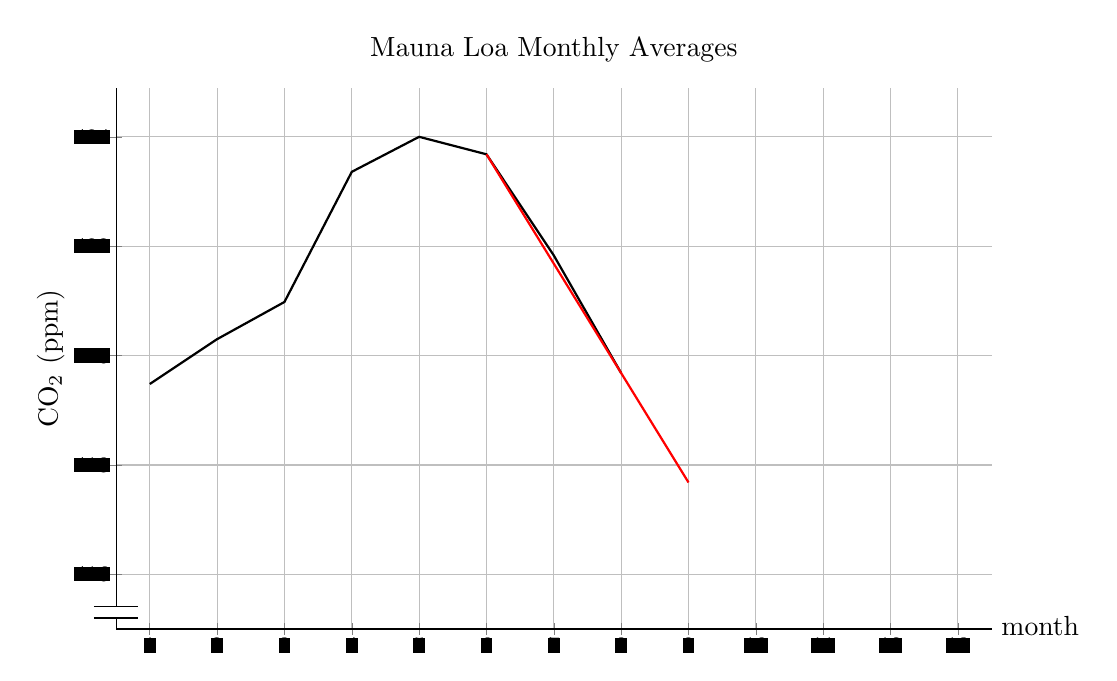
\begin{tikzpicture}
        \begin{axis}[xtick={1, 2, ..., 20}, ylabel=CO$_2$ (ppm), ylabel style={at=(ticklabel cs:0.5), anchor=south, text width=2.5in, align=center, rotate=90}, ticks=major, grid=major, axis line style={-}, title={Mauna Loa Monthly Averages}, axis y discontinuity=parallel, width=5in, height=3.33in, xlabel=month, xmin=0.5, xmax=13.5, ymin=415]
          \addplot[sharp plot] coordinates { (1, 419.48) (2, 420.3) (3, 420.98) (4, 423.36) (5, 424) (6, 423.68) (7, 421.83) (8, 419.68) };
          \solonly{
          \addplot[sharp plot, red] coordinates {(6, 423.68) (8, 419.68) (9, 417.68)};
          }
        \end{axis}
      \end{tikzpicture}
    \end{problem}

  \item

    \note{This prompts students to recognize that the slope is simply an average rate of change.}

    \begin{problem}[\vfill]
      In \ref{mauna-loa-reasonable}, you used a line to make an approximation. Explain what the slope of that line means; include units in your answer.
    \end{problem}

    \begin{solution}
      The slope of the line is
      \[\frac{419.68 - 423.68}{8-6} = -2,\]
      which represents the average rate of change of the CO$_2$ concentration with respect to time in ppm/month.
    \end{solution}

  \item 
    \begin{problem}[\vfill]
      Is it reasonable to use the line from (a) to predict the CO$_2$ concentration in January 2024? If so, find the predicted value; if not, explain why not.
    \end{problem}

    \begin{solution}
      It doesn't seem reasonable to assume that the CO$_2$ concentration is approximately linear on $[\text{June 2023}, \text{March 2024}]$; after all, we know that the CO$_2$ concentration typically decreases from May to October, then switches to increasing.
    \end{solution}

  \end{enumerate}

\item  \label{salmon-swimming-speed}

  \note{Here, I want students to try interpreting an average rate of change that's less intuitive. (This will also be important when we interpret derivatives.)

    When I interpret a rate of change, I like to give concrete examples. For instance, the average rate of change on $[15, 20]$ is about 1.4 cm/s per $^\circ$C, so if the temperature increases from 16$^\circ$C to $16.5^\circ$C, we'd expect the maximum swimming speed to increase by about (1.4 cm/s per $^\circ$C)($0.5^\circ$C).

    A common error in this problem is for students to say that the rate of change represents acceleration.

    If students are very uncomfortable with this and we have the time, I'll have them try \ref{AROC-ice-cream}.
  }

  \begin{problem}
    The maximum swimming speed of salmon depends on the water temperature. Suppose $S(T)$ is the maximum swimming speed (in cm/s) of salmon when the water temperature is $T$ degrees Celsius; the graph of $S$ is shown below. What does the average rate of change of $S$ on the interval $[15, 20]$ represent? What are its units?

    \begin{tikzpicture}[declare function={
        f(\x) = and(5 <= \x, \x <=15.4382) * (16.258900099989685 - 0.4500895572282921*\x + 0.028967810892554853*\x^2 + 0.0021388193107032267*\x^3)
        + and(15.4382 < \x, \x <=20.8213) * (-20.40986073953601 + 2.4878713424268084*\x + 0.10991422404638541*\x^2 - 0.005465637486958388*\x^3)
        + and(20.8213 < \x, \x <=27.236) * (-390.0944845580122 + 52.2220999074554*\x - 2.1091173263441054*\x^2 + 0.02734437354758604*\x^3)
        ;}]
      \begin{axis}[gridgraph, xmin=0, xmax=30, ymin=0, ymax=30, xtick={5,
          10, ..., 30}, ytick={5, 10, ..., 30}, 
        width=2.5in, height=1.5in] 
        \addplot+[domain=5:27.236] {f(x)};
      \end{axis}
    \end{tikzpicture}
  \end{problem}

  \begin{solution} 
    The average rate of change of $S$ on the interval $[15, 20]$ is $\frac{S(20) - S(15)}{20 - 15}$; the numerator has units of cm/s, while the denominator has units of $^\circ$C, so the average rate of change has units of \fbox{cm/s per $^\circ$C}. From the graph, we can see that $S(20) \approx 30$ and $S(15) \approx 23$, so this average rate of change is $\approx \frac{7}{5}$, or $\approx 1.4$ cm/s per $^\circ$C. What this means is that, when the temperature is around $15$ to $20^\circ$C, we expect each increase of $1^\circ$C to cause the salmons' maximum speed to increase by about $1.4$ cm/s. (For example, if the temperature were to increase from 16$^\circ$C to $16.5^\circ$C, we'd expect the salmons' maximum swimming speed to increase by about (1.4 cm/s per $^\circ$C)($0.5^\circ$C) = 0.7 cm/s.)
  \end{solution}

\item  \label{secant-approx}

  \note{We've now seen how secant line approximation can help us make predictions about the world, but there's another common use, which is to approximate mathematical expressions that are hard to calculate by hand.}

  \begin{enumerate}
  \item
    \begin{problem}
      \emph{Reminder:} $\sqrt[3]{x}$ can also be written as $x$ raised
      to what power?
    \end{problem}

    \begin{solution}
      $\sqrt[3]{x}=x^\frac{1}{3}$
    \end{solution}

  \end{enumerate}
  Here's the graph of $f(x) = \sqrt[3]{x}$ on $[0, 30]$. 

  \begin{tikzpicture}
    \begin{axis}[xtick=\empty, ytick=\empty, width=3.5in, height=2in]
      \addplot+[domain=0:1] {x^(1/3)};%
      \addplot+[domain=1:30] {x^(1/3)};%
    \end{axis}
  \end{tikzpicture}

  \begin{enumerate}[resume]

  \item \label{secant-line-approx-of-cube-root-10}

    \note{Here, we have to decide what secant line to look for. The most important thing is to pick 2 points that we can evaluate by hand. Here, we could use the secant line between $x = 8$ and $x = 27$ or the secant line between $x = 1$ and $x = 8$.

      As a default, encourage students to use the former, where the value of interest ($x = 10$) is between the values you're using.}

    \begin{problem}[\vfill]
      Use an appropriate secant line to approximate 
      $\sqrt[3]{10}$ by hand. Illustrate your approximation on the graph. 
    \end{problem}

    \begin{solution}
      To estimate $f(10)$, we can use a secant line between two nearby points whose $y$-values we can evaluate by hand.
      In this case, we know $f(8)=2$ and $f(27)=3$. (We could have also used $f(1)=1$, but we will typically pick
      points such that the value we want to approximate lies in between the points.)
    
      The average rate of change between $x=8$ and $x=27$ is $\frac{f(27) - f(8)}{27-8} =
      \frac{3 - 2}{19} = \frac{1}{19}$. This is the slope of the secant line pictured below in red.

      \begin{tikzpicture}
        \begin{axis}[xtick={8, 27}]
          \addplot+[domain=0:32] {x^(1/3)};
          \addplot+[domain=0:32] [red] {2 + (x - 8) / 19};
        \end{axis}
      \end{tikzpicture} 
      
      We know that the slope of the secant line is $\frac{1}{19}$. Using point-slope formula we can find the equation of the secant line.
      $$y-2 = \frac{1}{19} (x-8)$$
      $$ y = \frac{1}{19}(x-8) +2$$ 
      Now we use the line to estimate $\sqrt[3]{10}$.
      $$\sqrt[3]{10} \approx \frac{1}{19}(10-8) +2$$ 
      $$ \sqrt[3]{10} \approx \frac{2}{19}+2$$
      $$ \sqrt[3]{10} \approx \frac{40}{19} \approx 2.1$$ 
    \end{solution}

  \item

    \note{This is the last part I want to be sure to get to.}

    \begin{problem}[\stretch{0.25}]
      Is your estimate an overestimate (too high) or an underestimate (too low)?  How can you be sure? 
    \end{problem}

    \begin{problem}
      Another way we can say this is that a(n) \fitb{1in}{lower} bound for $\sqrt[3]{10}$ is 
      $\fitb{0.5in}{\frac{40}{19}}$.
    \end{problem}

    \begin{solution}
      We know our estimate is an underestimate because the secant line we drew
      lies below the graph of $y=\sqrt[3]{x}$ at $x=10$.
    \end{solution}

  \item
    \begin{problem}[\vfill]
      Use the secant line that you found in \ref{secant-line-approx-of-cube-root-10} to estimate $\sqrt[3]{7.5}$. Is your estimate too high or too low? 
    \end{problem}

    \begin{problem}      
      In other words, a(n) \fitb{1in}{upper} bound for $\sqrt[3]{7.5}$ is $\fitb{0.5in}{\frac{77}{38}}$.
    \end{problem}

    \begin{solution}
      The equation of the secant line we found previously was
      \[y=\frac{1}{19}(x-8)+2.\]
      Plugging in $x=7.5$, we can estimate that
      \begin{align*}
        \sqrt[3]{7.5} & \approx \frac{1}{19}(7.5-8) + 2 \\[2pt]
        & = \frac{1}{19}(0.5) + 2 \\[2pt]
        &= \frac{77}{38}.
      \end{align*}
      We know our estimate is an overestimate because the secant line we drew
      lies below the graph of $y=\sqrt[3]{x}$ at $x=7.5$.
    \end{solution}

  \item 

    \note{Just to emphasize that point-slope form is more useful here.} 

    \begin{problem}[\nstretch{0.35}]
      \emph{Reflect.} What form of the equation for a line was most
      useful in this problem?
    \end{problem}

    \begin{solution}
        Point-slope form was the most useful in this problem. We didn't need to find the $y$-intercept to write
        the equation of the line, and we were plugging in $x$-values which
        were around $x=8$, so $x-8$ was easy to work with.
    \end{solution}

  \end{enumerate}

  \item 
  \note{And this is just algebra practice in preparation for next class.}

  Let $f(x) = x^2 - x$.

  \begin{enumerate}
  \item \label{compute-AROC-with-h}
    \begin{problem}[\stretch{1.5}]
      Find the average rate of change of $f(x)$ between $x = 3$ and $3 + h$, where $h \neq 0$. (Should your answer involve $h$? How about $x$?) 
    \end{problem}

    \begin{solution}
      Using the definition of average rate of change,
      \begin{align*}
        \frac{f(3+h)-f(3)}{(3+h) - 3} &= \frac{\left((3+h)^2 - (3+h)\right) - \left(3^2 - 3\right)}{(3+h)-3} \\[2pt]
        &= \frac{9+6h+h^2 - (3+h) - 6}{h} \\[2pt]
        &= \frac{5h + h^2}{h} \\[2pt]
        &= 5 + h,\, h \neq 0.
      \end{align*}
    \end{solution}

  \item
    \begin{problem}[\nstretch{0.5}]
      Does your answer to \ref{compute-AROC-with-h} work when $h < 0$? 
    \end{problem}

    \begin{solution}
        Yes, the answer still works when $h$ is negative. However, $h$ cannot be zero.
    \end{solution}

  \end{enumerate}

\item 

  \note{This problem is preparing students to think about derivatives next class. If we get to it, I hope that students will think of looking at an average velocity between two times very close to 5. If there's time, we'll talk about how one way of doing this is to look at the average velocity between $5$ and a time very close to $5$, which we could call $5 + h$ where $h$ is very close to 0.}

  A rocket is launched straight up into the air. Suppose the function $f(t) = t^2$ describes the rocket's height in meters $t$ seconds after liftoff, and we'd like to know the rocket's \emph{instantaneous} velocity $5$ seconds after liftoff. That is, we'd like to know how fast the rocket is going right at the instant $t = 5$.

  \begin{enumerate}
  \item

    \begin{problem}[\vfill]
      We don't know how to find this instantaneous velocity exactly. Instead, come up with a good estimate for this velocity, and explain how you came up with your estimate.
    \end{problem}

    \begin{solution}
      To estimate the instantaneous velocity at $t=5$, we can calculate an average velocity between $t=5$ and 
      a time very close to $t=5$, let's say $t=5.1$. Using $f(t)=t^2$,
      \begin{align*}
          v_\text{avg} &= \frac{f(5.1)-f(5)}{5.1-5} \\[2pt]
          &= \frac{5.1^2 - 5^2}{5.1-5} \\[2pt]
          &= \frac{26.01 - 25}{5.1 - 5} \\[2pt]
          &= \frac{1.01}{0.1} \\[2pt]
          &= 10.1\text{ m/s}.
      \end{align*}
    \end{solution}

  \item

    \begin{problem}[\vfill]
      Can you think of a way to make your estimate even better? 
    \end{problem}

    \begin{solution}
      We could use an even shorter time interval, e.g. between $t=5$ and $t=5.01$. 
    \end{solution}

  \end{enumerate}



\item  \label{AROC-ice-cream}

  \note{Extra practice in case students were uncomfortable with anything from earlier in class}

  An ice cream shop is keeping track of how their sales are affected by price changes. When they sell a single scoop of ice cream for \$4, they sell 600 single scoops in a day. When they raise the price to \$4.50, they sell 560 single scoops in a day.

  Let $S(p)$ be the number of single scoops they sell in a day when the price is $\$p$.

  \begin{enumerate}
  \item
    \begin{problem}[1in]
      What does the average rate of change of $S(p)$ on $[4, 4.5]$ represent? What are its units?
    \end{problem}

    \begin{solution}
      The average rate of change is $\frac{S(4.5)-S(4)}{4.5-4}=\frac{560-600}{0.5}=-80$. 
      The numerator has units of scoops, and the denominator has units of dollars, 
      so the units of the average rate of change are \fbox{scoops per dollar.} It means that,
      when the price of ice cream is around \$4 to \$4.50, we would expect every \$1 increase in the price of ice cream
      to result in a decrease in the number of scoops sold by about 80.
    \end{solution}

  \item
    \begin{problem}
      Do you think it's reasonable to use local linearity to approximate the number of scoops the ice cream shop would sell if they changed the price of a scoop to \$4.20? How about if they changed the price to \$10?
    \end{problem}

    \begin{solution}
      It would be reasonable to use local linearity to approximate the number of scoops at a price of \$4.20,
      because the observed trend is not likely to change drastically on the interval between \$4 and \$4.50.
      However, it would not be reasonable to use information about sales when prices are around \$4 to estimate
      sales when the price is \$10. 
    \end{solution}

  \end{enumerate}

\end{enumerate}
\end{document}
